%& -shell-escape -enable-write18 
\documentclass[uplatex,dvipdfmx]{jsarticle}
\usepackage[utf8]{inputenc}

\usepackage[dvipdfmx]{graphicx}
\usepackage[dvipdfmx]{color}
\usepackage[driver=dvipdfm,hmargin=19.05truemm,vmargin=25.40truemm]{geometry}
\usepackage{colortbl}
\usepackage{tcolorbox}
\usepackage{varwidth}
\usepackage{xcolor}
\PassOptionsToPackage{dvipsnames}{xcolor}

\usepackage{amsmath,amsfonts,amssymb,amsthm}
\usepackage{bm}
\usepackage[italicdiff]{physics}
\usepackage{mathtools}
\mathtoolsset{showonlyrefs=true}
\usepackage[unicode, dvipdfmx]{hyperref}
\usepackage{pxjahyper}
\hypersetup{
setpagesize=false,
    bookmarksnumbered=true,
    bookmarksopen=true,
    colorlinks=true,
    linkcolor=cyan,
    citecolor=red,
}
\usepackage{mathrsfs}
\usepackage{bussproofs}
\usepackage{enumerate}
\usepackage{pxrubrica}
\usepackage{tipa}
\usepackage{ascmac}
\usepackage{caption}
\usepackage[subrefformat=parens]{subcaption}
\usepackage{listings,jvlisting}
\usepackage{tikz}
\usetikzlibrary{math,patterns,intersections,calc,arrows,graphs}
\usepackage{float}
\usepackage{xparse}
\usepackage{url}
\usepackage{fancyhdr}
\usepackage{multicol}
\usepackage{siunitx}
\usepackage{hhline}
\usepackage{bxbase}
\usepackage[mark=***]{sectionbreak}
\usepackage[geometry]{ifsym}
\usepackage[prefernoncjk]{pxcjkcat}
\usepackage[LGR,T2A,T3,T1]{fontenc}
\usepackage[greek,latin,english,russian,japanese]{pxbabel}

\allowdisplaybreaks


\theoremstyle{definition}
\newtheorem{theorem}{Thm}
\newtheorem{corollary}{Col}
\newtheorem{lemma}{Lem}
\newtheorem{definition}{Def}
\newtheorem{proposition}{Prop}

\tcbuselibrary{most}

\renewcommand{\labelitemi}{$\circ$}
\renewcommand{\labelitemii}{$\triangleright$}

\ProvideDocumentCommand\floor{m}{\lfloor {#1} \rfloor}
\ProvideDocumentCommand{\where}{}{\mathrel{}\middle|\mathrel{}}
\ProvideDocumentCommand{\when}{m}{\quad({#1})}
\ProvideDocumentCommand{\adjoint}{}{\mathbf{\ast}}
\ProvideDocumentCommand{\conjugation}{}{\mathbf{\ast}}
\NewDocumentCommand{\Jacobi}{m m}{\frac{\partial ({#1})}{\partial ({#2})}}
\NewDocumentCommand{\JacobiPolar}{O{x,y}}{\frac{\partial ({#1})}{\partial (r,\theta)}}
\DeclareMathOperator{\Ker}{Ker}
\DeclareMathOperator{\Img}{Im}
\DeclareMathOperator{\res}{Res}
\DeclareMathOperator{\Dom}{Dom}
\DeclareMathOperator{\Ran}{Ran}

\DeclareMathOperator{\exd}{d}

\DeclareFontShape{JY2}{mc}{m}{it}{<->ssub*mc/m/n}{}
\DeclareFontShape{JY2}{mc}{m}{sl}{<->ssub*mc/m/n}{}
\DeclareFontShape{JY2}{mc}{m}{sc}{<->ssub*mc/m/n}{}
\DeclareFontShape{JY2}{gt}{m}{it}{<->ssub*gt/m/n}{}
\DeclareFontShape{JY2}{gt}{m}{sl}{<->ssub*gt/m/n}{}
\DeclareFontShape{JY2}{mc}{b}{it}{<->ssub*mc/bx/it}{}
\DeclareFontShape{JY2}{mc}{bx}{it}{<->ssub*gt/m/n}{}
\DeclareFontShape{JY2}{mc}{bx}{sl}{<->ssub*gt/m/n}{}
\DeclareFontShape{JT2}{mc}{m}{it}{<->ssub*mc/m/n}{}
\DeclareFontShape{JT2}{mc}{m}{sl}{<->ssub*mc/m/n}{}
\DeclareFontShape{JT2}{mc}{m}{sc}{<->ssub*mc/m/n}{}
\DeclareFontShape{JT2}{gt}{m}{it}{<->ssub*gt/m/n}{}
\DeclareFontShape{JT2}{gt}{m}{sl}{<->ssub*gt/m/n}{}
\DeclareFontShape{JT2}{mc}{b}{it}{<->ssub*gt/b/n}{}
\DeclareFontShape{JT2}{mc}{bx}{it}{<->ssub*gt/m/n}{}
\DeclareFontShape{JT2}{mc}{bx}{sl}{<->ssub*gt/m/n}{}

\DeclareFontShape{J30}{mc}{b}{it}{<->ssub*mc/bx/it}{}
\DeclareFontShape{J30}{mc}{b}{n}{<->ssub*mc/bx/n}{}
\DeclareFontShape{J20}{mc}{b}{it}{<->ssub*mc/bx/it}{}
\DeclareFontShape{J20}{mc}{b}{n}{<->ssub*mc/bx/n}{}
\ProvideDocumentCommand{\titleof}{m}{

\title{ここに講義タイトルを入力 \\ {#1}レポート課題}
\author{ここに名前を入力}
\date{}
}

\titleof{12/07}

\begin{document}
    
\maketitle

\begin{enumerate}[(1)]
    
    \item $\Omega$は図\ref{fig:Omega}の橙色で塗られた領域で,赤色の境界を含む.
    \begin{figure}[H]
        \centering
        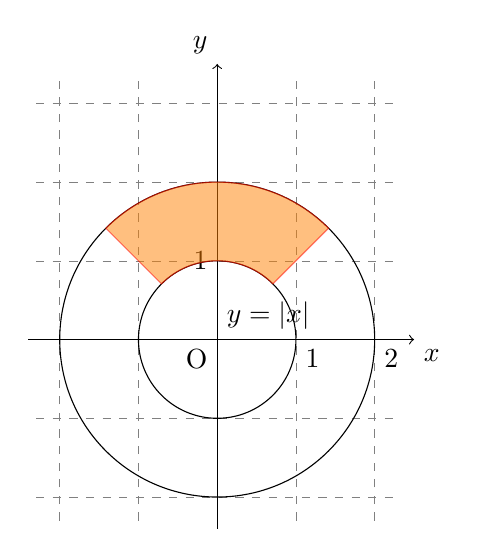
\begin{tikzpicture}[domain=1:1, yscale=1, xscale=1]
            
            \draw[very thin, dashed,color=gray] (-2.3,-2.3) grid (2.3,3.3);

            \draw[->] (-2.4,0) -- (2.5,0) node[below right] {$x$};
            \draw[->] (0,-2.4) -- (0,3.5) node[above left] {$y$};
            
            \draw (0,0) node[below left] {$\mathrm{O}$};
            \draw (1,0) node[below right] {$1$};
            \draw (2,0) node[below right] {$2$};
            \draw (0,1) node[left] {$1$};

            \draw (0,0) circle [radius=1]; 
            \draw (0,0) circle [radius=2]; 
            \draw[domain=-2.3:2.3] plot function{abs(x)} node[above right] {$y=\abs{x}$};

            \filldraw[fill=orange,opacity=.5,draw=red] (45:1) -- (45:2) arc (45:135:2) -- (135:1) arc (135:45:1);
        \end{tikzpicture}
        \caption{領域$\Omega$}
        \label{fig:Omega}
    \end{figure}
    $\Omega$を極座標表示すると,
    \begin{equation}
        \Omega : \qty{ \qty( r\cos \theta, r \sin \theta ) \where 1\le r \le 2, \frac{\pi}{4}\le \theta \le \frac{3}{4}\pi}
    \end{equation}
    であるから
    \begin{align}
        \iint_\Omega x^2y\dd{x}\dd{y}
        &= \iint_\Omega (r\cos \theta)^2(r \sin \theta)\abs{\Jacobi{x,y}{r,\theta}} \dd{r}\dd{\theta}\\
        &= \iint_\Omega r^4\cos^2 \theta\sin \theta\dd{r}\dd{\theta}\\
        &= \int^2_1 r^4\dd{r}\int^{\frac{3}{4}\pi}_{\frac{\pi}{4}} \cos^2 \theta\sin \theta\dd{\theta}\\
        &= \eval[\frac{1}{5}r^5|^{2}_{1} \eval[-\frac{1}{3}\cos^3 \theta |^{\frac{3}{4}\pi}_{\frac{\pi}{4}}\\
        &= \frac{31}{5}\cdot \qty(-\frac{1}{3})\cdot\qty(-\frac{2}{\sqrt{2}^3})\\
        &= \frac{31}{15\sqrt{2}}
    \end{align}
    である.
    \item 
    \begin{enumerate}[(i)]
        \item 
        \begin{equation}
            \begin{dcases}
                u&=\frac{1}{\sqrt{2}}(s-t)\\
                v&=\frac{1}{\sqrt{2}}(s+t)
            \end{dcases}
        \end{equation}
        とすると$(s,t),(u,v)$の対応は全単射である($\because$原点を中心とした回転なので).$\Phi((s,t))=(x_0,y_0)$のとき
        \begin{align}
            &\begin{dcases}
                s^2+t^2&=x_0\\
                st&=y_0
            \end{dcases}\\
            \therefore
            &\begin{dcases}
                u^2+v^2&=x_0\\
                -u^2+v^2&=2y_0
            \end{dcases}\label{eq:1}
        \end{align}
        である.$t_0\ne\pm s_0$ゆえ$u\ne 0$.
        \eqref{eq:1}式の$u> 0\land v\ge 0$の部分を見ると,

        $v=\sqrt{x_0 - u^2}$は$u$に関して単調減少,$v=\sqrt{2y_0 + u^2}$は$u$に関して単調増加なので,
        \begin{equation}
            \sqrt{x_0 - u^2}=\sqrt{2y_0 + u^2}
        \end{equation}
        となる$u$は存在すれば一意である.そのような$u$として
        \begin{equation}
            u=\frac{1}{\sqrt{2}}(s_0-t_0)
        \end{equation}
        があり,これに限る.
        \eqref{eq:1}式は$u=0,v=0$に関して対称なので,結局,\eqref{eq:1}式を満たす$(u,v)$の組は
        \begin{equation}
            (u,v) 
            = \qty(\pm \frac{1}{\sqrt{2}}(s_0-t_0), \pm \frac{1}{\sqrt{2}}(s_0+t_0))\qq{(複号任意)}
        \end{equation}
        の4つである.すなわち,$\Phi((s,t))=(x_0,y_0)$となる$(s,t)$の組は
        \begin{equation}
            (s,t) 
            = \qty(\pm s_0, \pm t_0)\qq{(複号同順)},\qty(\pm t_0, \pm s_0)\qq{(複号同順)}
        \end{equation}
        の4つである.
        \begin{figure}[H]
            \centering
            \begin{tikzpicture}[domain=1:1, yscale=1, xscale=1]
                \draw[->] (-2.1,0) -- (2.2,0) node[below right] {$u$};
                \draw[->] (0,-2.1) -- (0,2.2) node[above left] {$v$};
                
                \draw (0,0) node[below left] {$\mathrm{O}$};
                \draw (1,0) node[below right] {$\sqrt{x_0}$};
                \draw (0,0.6) node[below left] {$\sqrt{2y_0}$};

                \draw[name path=cir, color=cyan] (0,0) circle [radius=1] (1,0) node[above right] {$u^2+v^2=x_0$}; 
                \draw[name path=hyp1, color=red, domain=-2.0:2.0] plot function{sqrt(x**2+0.6)} node[above right] {$-u^2+v^2=2y_0$の上枝};
                \draw[name path=hyp2, color=red, domain=-2.0:2.0] plot function{-sqrt(x**2+0.6)} node[above right] {$-u^2+v^2=2y_0$の下枝};

                \fill[name intersections={of= cir and hyp1, name=i, total=\t}][color=magenta, opacity=0.5] \foreach \s in {1,...,\t}{(i-\s) circle (2pt) }; 
                \fill[name intersections={of= cir and hyp2, name=i, total=\t}][color=magenta, opacity=0.5] \foreach \s in {1,...,\t}{(i-\s) circle (2pt) }; 
            \end{tikzpicture}
            \caption{$uv$平面上で見た\eqref{eq:1}式}
            \label{pic:uv}
        \end{figure}
        \item \begin{align}
            \Jacobi{x,y}{s,t}
            &=\mqty|
                \pdv*{x}{s} & \pdv*{x}{t}\\
                \pdv*{y}{s} & \pdv*{y}{t}
                |\\
            &=\mqty|
                2s & 2t\\
                t & s
                |\\
            &=2(s^2-t^2)
        \end{align}
        である.
        \item 
        \begin{align}
            D&=\qty{(s,t)\where \abs{s}+\abs{t}\le 4}\\
            D_1&=D\cap \qty{(s,t)\where \frac{1}{\sqrt{2}}(s-t)\ge 0\land \frac{1}{\sqrt{2}}(s+t)\ge 0}
        \end{align}
        とおくと,(i)で確かめたことより
        \begin{equation}
            S=\Phi(D)=\Phi(D_1)
        \end{equation}
        であり,しかも
        \begin{equation}
            E=D_1\cap \qty{(s,t)\where \frac{1}{\sqrt{2}}(s-t)= 0\lor \frac{1}{\sqrt{2}}(s+t)= 0}
        \end{equation}
        とすると$m(E) =0$で,$D_1\setminus E$上で
        $\Jacobi{x,y}{s,t}\ne 0$となり単射.ゆえに
        \begin{equation}
            \Phi|D_1 : D_1 \to S
        \end{equation}
        はほぼ全単射である.

        また,
        \begin{equation}
            \begin{dcases}
                s&=\frac{1}{\sqrt{2}}(u+v)\\
                t&=-\frac{1}{\sqrt{2}}(u-v)
            \end{dcases}
        \end{equation}
        で$uv$平面から$st$平面への対応$\Psi$を定め,
        \begin{equation}
            W=\qty{(u,v)\where 0\le u, v \le 2\sqrt{2}}
        \end{equation}
        とおくと,$\Psi|W:W\to D_1$は全単射なので
        \begin{align}
            m(S)
            &=\iint_S \dd{x}\dd{y}\\
            &=\iint_{D_1} \Jacobi{x,y}{s,t} \dd{s}\dd{t}\\
            &=\iint_W \Jacobi{s,t}{u,v} \Jacobi{x,y}{s,t} \dd{u}\dd{v}\\
            &=\int^{2\sqrt{2}}_0 \qty(\int^{2\sqrt{2}}_0 4uv \dd{u})\dd{v}\\
            &=\int^{2\sqrt{2}}_0 16v\dd{v}\\
            &=64
        \end{align}
        である.
    \end{enumerate}
    \item 
    \begin{enumerate}[(i)]
        \item 以下ではFubiniの定理を断りなく使う.
        \begin{equation}
            I=\iint_\Omega\cos(2\pi(x+y))dxdy,
            J=\iint_\Omega\sin(2\pi(x+y))dxdy
        \end{equation}
        とおく.
        \begin{itemize}
            \item $b - a \in \mathbb{Z} \lor d - c \in \mathbb{Z}$のとき
            \begin{itemize}
                \item $b - a \in \mathbb{Z}$のとき
                \begin{align}
                    I
                    &=\int^d_c \qty(\int^b_a \cos(2\pi(x+y))dx) dy\\
                    &=\int^d_c 0\cdot dy\\
                    &=0\\
                    J
                    &=\int^d_c \qty(\int^b_a \sin(2\pi(x+y))dx) dy\\
                    &=0\\
                    \therefore
                    I&=J=0
                \end{align}
                \item $d - c \in \mathbb{Z}$のとき
                \begin{align}
                    I
                    &=\int^b_a \qty(\int^d_c \cos(2\pi(x+y))dy) dx\\
                    &=\int^b_a 0\cdot dx\\
                    &=0\\
                    J
                    &=\int^b_a \qty(\int^d_c \sin(2\pi(x+y))dy) dx\\
                    &=0\\
                    \therefore
                    I&=J=0
                \end{align}
                よって,いずれの場合も
                \begin{equation}
                    I=J=0
                \end{equation}
                である.
            \end{itemize}
            \item $b - a \notin \mathbb{Z} \land d - c \notin \mathbb{Z}$のとき
            \begin{align}
                I
                &=\int^d_c \qty(\int^b_a \cos(2\pi(x+y))dx) dy\\
                &=\int^d_c \frac{1}{2\pi} \eval[\sin(2\pi(x+y)) |^b_{x\coloneqq a} dy\\
                &=\frac{1}{2\pi} \int^d_c \qty(\sin(2\pi(y+b))- \sin(2\pi(y+a))) dy\\
                &=\frac{1}{\pi} \int^d_c \cos(2\pi(y+\frac{a+b}{2}))\sin(\pi(b-a)) dy\\
                &=\frac{\sin(\pi(b-a))}{\pi} \int^d_c \cos(2\pi(y+\frac{a+b}{2})) dy\\
                &\ne 0
            \end{align}
            である.
        \end{itemize}
        以上から
        \begin{equation}
            I=J=0 \Longleftrightarrow  b - a \in \mathbb{Z} \lor d - c \in \mathbb{Z}
        \end{equation}
        が示された.
        \item \
        \begin{theorem}
            もとの長方形ABCDのたてまたはよこの少なくとも一方の長さは必ず有理数であるといえる.
        \end{theorem}
        \begin{proof}
            長方形$ABCD$を$xy$平面上で表したものを$\Omega_0$とし,
            \begin{equation}
                \Omega_0=\qty{(x,y)\where a_0\le x \le b_0\land c_0 \le y \le d_0}
            \end{equation}
            となるように文字をおく.
            
            また,長方形$ABCD$を分割した小長方形は,分割した個数を$n$,$1\le i \le n$として
            \begin{equation}
                \Omega_i=\qty{(x,y)\where a_i\le x \le b_i\land c_i \le y \le d_i} 
            \end{equation}
            とおける.各$i$について,$b_i-a_i, d_i-c_i$の少なくとも1つは有理数であるから,それを整数/整数の形で表したときの分母を$q_i$とする.
            
            さて,$\Omega_i$を$\displaystyle q=\prod_{1\le i \le n} q_i$倍に拡大したもの,すなわち
            \begin{equation}
                \Xi_i = \qty{(x,y)\where a_iq\le x \le b_iq\land c_iq \le y \le d_iq} 
            \end{equation}
            として,$\Xi_i$で$\cos(2\pi(x+y)),\sin(2\pi(x+y))$を積分することを考える.いま,$b_iq - a_iq, d_iq - c_iq$の少なくとも一方が整数なので,(i)の結果より
            \begin{equation}
                \iint_{\Xi_i} \cos(2\pi(x+y))dxdy
                =\iint_{\Xi_i} \sin(2\pi(x+y))dxdy
                =0
            \end{equation}
            である.そして,$m(\Omega_i \cap \Omega_j) =0 \quad (i\ne j)$であるので,$m(\Xi_i \cap \Xi_j) =0 \quad (i\ne j)$である.よって,
            \begin{align}
                \Xi_0 
                &= \bigcap_{1\le i \le n} \Xi_i
                = \qty{(x,y)\where a_0q\le x \le b_0q\land c_0q \le y \le d_0q} 
            \end{align}
            とおくと,
            \begin{align}
                \iint_{\Xi_0} \cos(2\pi(x+y))dxdy
                &=\sum_{i=1}^n \iint_{\Xi_i} \cos(2\pi(x+y))dxdy
                =0,\\
                \iint_{\Xi_0} \sin(2\pi(x+y))dxdy
                &=\sum_{i=1}^n \iint_{\Xi_i} \sin(2\pi(x+y))dxdy
                =0
            \end{align}
            となる.(i)の結果より,
            
            \begin{equation}
                b_0q - a_0q, d_0q - c_0q\text{のうち少なくとも一方が整数}
            \end{equation}
            すなわち
            \begin{equation}
                b_0 - a_0\text{(=たて(resp. よこ)の長さ)}, d_0 - c_0\text{(=よこ(resp. たて)の長さ)}\text{のうち少なくとも一方が有理数}
            \end{equation}
            が従う.以上で示された.
        \end{proof}

    \end{enumerate}
    
\end{enumerate}

\end{document}